\section{The Game Deserved Score Framework}
\label{sec:gds}

\subsection{Motivation: The Noisiness of Point Differential}

The most common summary statistic of NFL game performance is point differential:
the margin of victory or defeat at the final whistle. Point differential is
intuitively appealing and correlates with season outcomes at the aggregate
level \parencite{stern1991probability}, but it is a poor measure of within-game
performance quality. Scoring
events in American football are discrete and lumpy \parencite{lopez2018randomness}; a single play can produce
seven points while an extended drive producing sustained field position may
produce none. As a result, the final score frequently fails to reflect which
team controlled the game's probabilistic narrative.

Analysis of the 2018--2024 NFL seasons in the present study confirms this
systematically: approximately 25\% of regular-season games are won by the team
that gained fewer yards and converted fewer first downs than its opponent. Teams can -- and
frequently do -- lose the statistical battle while winning the scoreboard battle
through turnover returns, short fields, special teams scores, or simply higher
variance in the timing of their offensive execution. A team that accumulates
eight field-goal opportunities and converts three is not straightforwardly
inferior to a team that accumulates two touchdown opportunities and converts
both; yet point differential records only the nine-point and fourteen-point
outcomes and treats them identically regardless of the underlying process.

This motivates a framework that decomposes game-level performance into the
contributions of the underlying offensive, defensive, and special teams
processes, evaluated in a common unit that is directly comparable across games
and teams. The Game Deserved Score (\gds{}) framework serves this purpose.
\Cref{fig:pipeline} provides a schematic overview of the end-to-end
computation pipeline.

\begin{figure}[htbp]
  \centering
  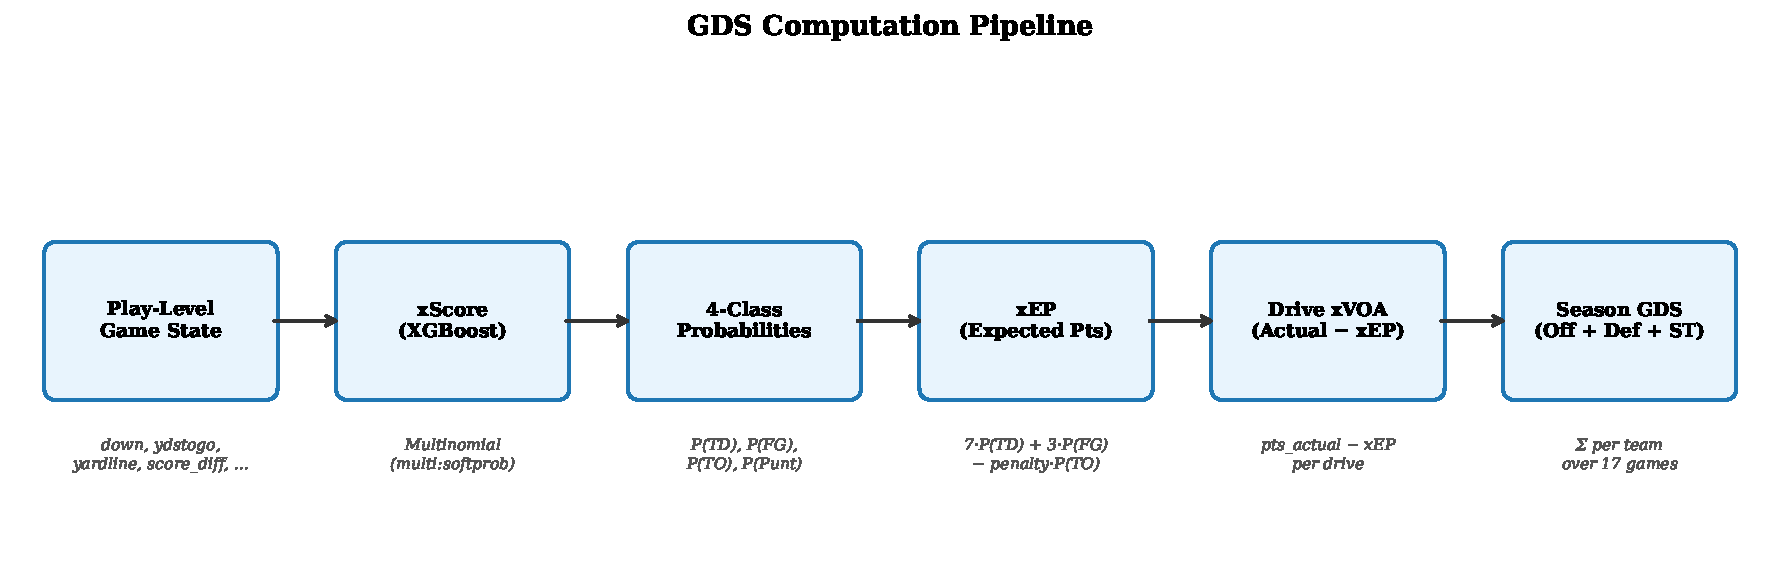
\includegraphics[width=\textwidth]{figures/fig9_pipeline_flowchart.pdf}
  \caption{End-to-end GDS computation pipeline. Situational game-state features
           feed into the multinomial \xscore{} model, producing four-class drive
           outcome probabilities that are converted to expected points (xEP).
           Drive-level value over average (xVOA) is aggregated to season-level
           GDS decomposed into offensive, defensive, and special-teams
           contributions.}
  \label{fig:pipeline}
\end{figure} The
central idea is analogous to the Expected Possession Value decomposition in
basketball analytics: rather than asking ``which team scored more?'', the
framework asks ``which team generated and suppressed scoring-probability at a
rate inconsistent with league expectations, and by how much?''
\parencite{cervone2016multiresolution}. The currency of this accounting is
the expected points value derived from the multinomial \xscore{} probability
vector introduced in \Cref{sec:xscore}: for each drive, the model's four-class
output is converted into a single expected-point figure representing what a
league-average team would score from the given situational state.

\subsection{Three-Component Decomposition}
\label{sec:gds-decomposition}

\gds{} decomposes game-level deserved performance into three additive channels:
offensive expected value over average (Off\_\xvoa{}), defensive expected value over average (Def\_\xvoa{}), and special teams value (ST\_Value).
The decomposition is exhaustive in the following sense: every drive in a game
is routed through exactly one of the three channels based on its scoring
outcome relative to the expected points at drive start.

\begin{itemize}
  \item \textbf{Offensive \xvoa{}} captures the degree to which the possession
        team's offensive execution generated points above or below the
        situational baseline. A team that consistently scored more points than
        expected from its drive-opening states accumulates positive offensive
        \xvoa{}.

  \item \textbf{Defensive \xvoa{}} captures the degree to which the defensive
        team suppressed the opponent's ability to generate points above
        expectation. It is derived directly from the opponent's offensive
        \xvoa{}, ensuring consistency of scale and eliminating the need for a
        separate defensive model.

  \item \textbf{Special Teams Value} (\textit{ST~Value}) captures the advantage
        or disadvantage conferred by the field position inherited at the start
        of each drive, relative to what that drive-start type typically yields
        across the league. It accounts for the value of returns, punting
        quality, kickoff coverage, and turnover field position in a unified
        framework.
\end{itemize}

The three channels partition every scoring-relevant action in the game. A
turnover that ends an offensive drive is penalized in offensive \xvoa{} (the
drive scores zero points against a positive expected-point baseline) and
rewarded in special teams value for the opponent (whose subsequent drive begins
at a superior starting position). A defensive stop that forces a three-and-out does not generate a
separate accounting entry; instead, it is reflected in the negative offensive
\xvoa{} of the opponent, which by the mirror formula (\Cref{sec:def-xvoa})
becomes a positive defensive \xvoa{} for the defending team. This structure
guarantees that no event is double-counted.

Formally, for a team $A$ in a game against opponent $B$, the Game Deserved
Score is defined as:

\begin{equation}
  \label{eq:gds}
  \gds(A) = \xvoa{}_{\mathrm{Off}}(A) + \xvoa{}_{\mathrm{Def}}(A)
             + \mathrm{ST}(A),
\end{equation}

where the three terms are defined and formalized in the subsections that
follow. All three terms are expressed in expected-point units: a
\gds{} of $+7.0$ means that the team generated the equivalent of one full
touchdown of net positive performance beyond what a league-average team
would have been expected to produce in identical circumstances.

\subsection{Offensive Value Added}
\label{sec:xvoa}

Offensive \xvoa{} measures the net difference between the points actually
scored on a drive and the expected points assigned to that drive's opening
state by the multinomial \xscore{} model (\Cref{sec:xscore}). The intuition
is straightforward: a drive that begins from a state where the model predicts
$\mathrm{xEP} = 2.1$ and ends in a touchdown (7 points) has generated $7 - 2.1
= 4.9$ points of value above expectation. A drive that begins from the same
state and ends in a punt (0 points) has generated $0 - 2.1 = -2.1$ points of
value relative to the baseline. The accumulated sum of these drive-level
differences across all of a team's possessions reflects the offensive
contribution that cannot be explained by the situational context alone.

This framing is analogous to the expected-goals framework in association
football analytics, where the accumulated difference between actual goals and
expected goals over a match captures shooting quality and finishing efficiency
beyond what shot location and context predict
\parencite{rathke2017expectedgoals}. In the present application, the outcome
space is expected points derived from the multinomial probability vector rather
than a single goal probability, and the accumulation occurs at the drive level
using actual points scored versus expected points at drive start.

\subsubsection{Drive-Level xVOA}

Under the multinomial model, offensive \xvoa{} is computed directly at the
drive level rather than through play-to-play deltas. Let $s_1^{(d)}$ denote
the situational state of the first play of drive $d$, and let
$\mathrm{xEP}(s_1^{(d)})$ be the expected points at that state as defined
in \Cref{eq:xep}. Let $\mathrm{pts}(d)$ denote the actual points scored on
drive $d$:

\begin{equation}
  \label{eq:pts-drive}
  \mathrm{pts}(d) =
    \begin{cases}
      7 & \text{if drive } d \text{ ends in an offensive touchdown}, \\
      3 & \text{if drive } d \text{ ends in a made field goal}, \\
      0 & \text{otherwise (punt, turnover, end of half, safety).}
    \end{cases}
\end{equation}

Safeties are classified under the zero-point category. Although a safety
yields two points for the \emph{defensive} team, the possession team's drive
scores zero; the opponent's two-point gain is captured through the subsequent
kickoff drive's starting field position, which enters the special teams
channel. Safeties occur on fewer than 0.5\% of drives, making their treatment
inconsequential to aggregate results.

The per-drive offensive value added is then the difference between actual
points and expected points:

\begin{equation}
  \label{eq:xvoa-drive}
  \xvoa{}^{(d)} = \mathrm{pts}(d) - \mathrm{xEP}\!\bigl(s_1^{(d)}\bigr).
\end{equation}

This formulation captures the full information content of the multinomial
model. A drive that begins in a state with $\mathrm{xEP} = 2.8$ (reflecting,
say, a 30\% TD probability, a 25\% FG probability, and moderate turnover risk)
and ends in a touchdown generates $\xvoa{}^{(d)} = 7 - 2.8 = +4.2$. The same
drive ending in a field goal generates $\xvoa{}^{(d)} = 3 - 2.8 = +0.2$ -- still
positive, reflecting that the team exceeded expectation, but capturing the
fact that a field goal from a favorable state represents only modest
overperformance. A drive ending in a punt generates $\xvoa{}^{(d)} = 0 - 2.8
= -2.8$, penalizing the failure to convert a state with substantial scoring
expectation. This graduated accounting -- distinguishing between a 7-point
outcome, a 3-point outcome, and a 0-point outcome -- is the primary advantage
of the multinomial approach over the binary model, which could only distinguish
between touchdown and not-touchdown.

\subsubsection{Game-Level Aggregation}

Offensive \xvoa{} for team $A$ in a game is the sum of per-drive values
across all of that team's drives in the game:

\begin{equation}
  \label{eq:xvoa-off}
  \xvoa{}_{\mathrm{Off}}(A) = \sum_{d \in \mathcal{D}(A)} \xvoa{}^{(d)}
    = \sum_{d \in \mathcal{D}(A)}
      \Bigl[\mathrm{pts}(d) - \mathrm{xEP}\!\bigl(s_{1}^{(d)}\bigr)\Bigr],
\end{equation}

where $\mathcal{D}(A)$ is the set of drives run by team $A$ in the game.
The interpretation is direct: offensive \xvoa{} is the aggregate difference
between actual points scored and the expected points that league-average
execution would have been expected to produce from the same sequence of
drive-opening states. A team that converts consistently above its situational
baseline accumulates positive offensive \xvoa{}; a team that fails to convert
from high-expected-point positions accumulates negative offensive \xvoa{}.

\subsection{Defensive Value Added}
\label{sec:def-xvoa}

A separate defensive probability model is not required in the \gds{} framework.
The defensive contribution of team $A$ in a game against team $B$ is defined
as the negative of the offensive \xvoa{} that team $B$ produced:

\begin{equation}
  \label{eq:xvoa-def}
  \xvoa{}_{\mathrm{Def}}(A) = -\,\xvoa{}_{\mathrm{Off}}(B).
\end{equation}

The logic is as follows. The offensive \xvoa{} of team $B$ measures the
aggregate points that team $B$'s offense generated beyond situational
expectation. Those points must have been generated against some defensive
unit -- and in a two-team game, that unit is team $A$'s defense. A high
offensive \xvoa{} for team $B$ therefore indicates that team $A$'s defense
was suppressed or beaten relative to what a league-average defense would have
allowed in the same situational sequence. Negating team $B$'s offensive \xvoa{}
converts this into a defensive penalty for team $A$. Symmetrically, if team $B$
generated negative offensive \xvoa{} (underperformed the situational baseline),
team $A$'s defense receives positive credit.

This mirror construction has two practical advantages. First, it guarantees
that the sum of offensive and defensive \xvoa{} contributions across both teams
in any single game is exactly zero: $\xvoa{}_{\mathrm{Off}}(A) +
\xvoa{}_{\mathrm{Def}}(B) + \xvoa{}_{\mathrm{Off}}(B) +
\xvoa{}_{\mathrm{Def}}(A) = 0$. The game-level \gds{} values for both teams
therefore differ only by the net effect of special teams play, which is not
in general zero-sum (both teams' special teams can add or subtract from
expected value independently). Second, the mirror construction avoids the
attribution ambiguity that would arise if defensive \xvoa{} were computed
directly from defensive plays (sacks, tackles for loss, pass deflections),
which overlap with the offensive drive sequence and would risk double-counting
plays that are already accounted for in the opponent's offensive \xvoa{}.

Positive defensive \xvoa{} means the defense held the opponent below its
expected offensive output. Negative defensive \xvoa{} means the defense
allowed the opponent to generate more points above expectation than the
league-average defense would have allowed against the same sequence of
situational states.

\subsection{Special Teams Value}
\label{sec:st-value}

Special teams play affects \gds{} through the starting field position it
confers at the beginning of each offensive drive. A kick returner who advances
a kickoff to the 35-yard line instead of the 25-yard line has, in effect,
transferred ten yards of field position to the subsequent possession -- which
the \xscore{} model will translate into higher starting expected points.
The Special Teams Value component quantifies this transfer.

\subsubsection{Drive Transition Types}
\label{sec:drive-transitions}

Each drive in the dataset is associated with a transition type that records
the event that initiated the possession. The raw \texttt{nflfastR} dataset
contains a richer set of transition labels, including rare variants such as
muffed punts, blocked kicks, and onside recoveries. These rare types are
consolidated into six canonical categories to ensure stable baseline
estimation:

\begin{table}[htbp]
  \centering
  \caption{Drive transition type taxonomy. Rare raw labels are consolidated
           into six canonical categories for stable baseline computation.}
  \label{tab:transitions}
  \small
  \begin{tabularx}{\textwidth}{l l X}
    \toprule
    \textbf{Canonical} & \textbf{Raw Subtypes} & \textbf{Description} \\
    \midrule
    \texttt{KICKOFF}
      & Kickoff, onside kick, muffed kickoff
      & Possession via any kickoff variant \\[3pt]
    \texttt{PUNT}
      & Punt, blocked punt, muffed punt
      & Possession via punt or blocked/muffed punt \\[3pt]
    \texttt{MISSED\_FG}
      & Missed FG, blocked FG, muffed FG
      & Possession via missed or blocked FG attempt \\[3pt]
    \texttt{INTERCEPTION}
      & Interception
      & Possession via forward pass interception \\[3pt]
    \texttt{FUMBLE}
      & Fumble
      & Possession via defensive fumble recovery \\[3pt]
    \texttt{DOWNS}
      & Downs
      & Possession via failed 4th-down conversion \\
    \bottomrule
  \end{tabularx}
\end{table}

The motivation for this consolidation is statistical stability. Rare events
such as blocked field goals occur fewer than thirty times per season across
the entire league; computing a reliable mean starting $\mathrm{xEP}$ from such
sparse samples requires either pooling with a parent category or accepting
high-variance estimates. The consolidation in \Cref{tab:transitions} groups
each rare type into the parent category that best matches its typical
starting field position, and the resulting canonical categories each contain
hundreds of drives in the training window.

\subsubsection{Baseline Computation}

The expected starting $\mathrm{xEP}$ for each canonical transition type is
estimated empirically from the training data (seasons 2018--2024) as the
arithmetic mean of the $\mathrm{xEP}$ value at the first play of all drives of
that type:

\begin{equation}
  \label{eq:st-baseline}
  \mu_{\tau} = \frac{1}{|\mathcal{D}_{\tau}|}
    \sum_{d \in \mathcal{D}_{\tau}} \mathrm{xEP}\!\bigl(s_1^{(d)}\bigr),
\end{equation}

where $\mathcal{D}_{\tau}$ is the set of all training-window drives that begin
with transition type $\tau$ drawn from the six canonical categories defined in
\Cref{tab:transitions}, and $s_1^{(d)}$ is the first play of drive $d$.

Several design choices in this formula warrant comment. First, the baseline
uses \emph{actual} $\mathrm{xEP}$ values at the observed first play rather than
a synthetic neutral state (e.g., a fixed yardline and down). This means that
the baseline implicitly captures the real game context in which each
transition type tends to occur: kickoffs, for instance, often occur
early in drives following scoring plays, when the clock situation and score
differential create a particular probabilistic context. The baseline is
therefore an empirical distribution over real game states, not a
stylized average.

Second, the baseline is computed once on the training window and held fixed
for all subsequent applications -- including the 2025 test set and any
out-of-distribution evaluation. This prevents leakage: the expected value
for a transition type on a given test play is derived only from training-window
data.

Third, individual drive first-play $\mathrm{xEP}$ values reflect the full
situational state (field position, down, distance, score differential, time),
so the baseline $\mu_\tau$ implicitly integrates over the typical game states
that accompany each transition type. A team that consistently receives good
kickoff returns will systematically start kickoff drives at a higher
$\mathrm{xEP}$ than $\mu_{\texttt{KICKOFF}}$, and this difference is credited
to special teams value.

\subsubsection{Per-Drive Special Teams Value}

For each drive $d$ with transition type $\tau(d)$, the per-drive special
teams value is the deviation of the actual starting $\mathrm{xEP}$ from the
type-specific baseline:

\begin{equation}
  \label{eq:st-drive}
  \mathrm{ST}^{(d)} = \mathrm{xEP}\!\bigl(s_1^{(d)}\bigr) - \mu_{\tau(d)}.
\end{equation}

A positive per-drive ST~value means the drive began from a more favorable
field position than the league average for that transition type. A negative
value means the drive began from a less favorable position.

\subsubsection{Game-Level Aggregation}

The game-level special teams value for team $A$ is the sum of per-drive
ST values across all drives in the game:

\begin{equation}
  \label{eq:st-game}
  \mathrm{ST}(A) = \sum_{d \in \mathcal{D}(A)} \mathrm{ST}^{(d)}.
\end{equation}

This formulation rewards teams that consistently secure superior starting
positions across all their drives -- regardless of whether those superior
positions were obtained via kick returns, punt coverage, or the opponent's
failed fourth-down attempts.

\subsection{Attribution Rules and Turnover Handling}
\label{sec:attribution}

A potential concern with any decomposition framework is double-counting:
could the same underlying play contribute to multiple components? The
structure of the \gds{} framework is designed to prevent this, and the
treatment of turnovers provides the clearest illustration.

When the offense commits a turnover -- an interception or fumble recovery by
the defense -- the following accounting occurs:

\begin{enumerate}
  \item \textbf{Offensive \xvoa{} of the turning team.} The drive containing
        the turnover terminates at $\mathrm{pts}(d) = 0$. The drive-level
        \xvoa{} is $0 - \mathrm{xEP}(s_1^{(d)})$, which is negative whenever
        the drive began from a state with positive expected points (as
        virtually all drives do). The full cost of the failed drive is
        absorbed by the turning team's offensive \xvoa{}.

  \item \textbf{Special teams value of the receiving team.} The opponent's
        subsequent drive begins with a transition type of
        \texttt{INTERCEPTION} or \texttt{FUMBLE}, and its starting
        $\mathrm{xEP}$ is compared to the $\mu_{\texttt{INTERCEPTION}}$ or
        $\mu_{\texttt{FUMBLE}}$ baseline. Turnovers often occur near midfield
        or in opposition territory, so the receiving team frequently begins
        from a higher-than-average starting position for that transition type,
        generating positive special teams value. However, this credit goes only
        to the starting field position advantage -- not to the act of forcing
        the turnover itself.

  \item \textbf{Defensive \xvoa{} of the receiving team.} The receiving team's
        defensive \xvoa{} is the negative of the turning team's offensive
        \xvoa{} -- which, as established in point~1, already accounts for the
        failed drive including the turnover. No additional defensive entry is
        created for the turnover play.
\end{enumerate}

The result is a clean partition: the cost of the turnover is borne entirely
by the turning team's offensive channel; the positional benefit of the
resulting field position is credited to the receiving team's special teams
channel; and the defensive channel receives credit for the overall
suppression of the opponent's offensive \xvoa{} without any separate
entry for the turnover event. No play is counted in more than one channel.

\subsection{Formal Properties of \gds{}}
\label{sec:gds-properties}

The \gds{} framework satisfies several formal properties that support its
use as an analytical tool.

\paragraph{Zero-sum decomposition.}
For any single game between teams $A$ and $B$:
\begin{equation}
  \label{eq:zero-sum}
  \bigl[\xvoa{}_{\mathrm{Off}}(A) + \xvoa{}_{\mathrm{Def}}(A)\bigr]
  +
  \bigl[\xvoa{}_{\mathrm{Off}}(B) + \xvoa{}_{\mathrm{Def}}(B)\bigr]
  = 0.
\end{equation}
This follows directly from the mirror definition in \Cref{eq:xvoa-def}:
\begin{align*}
  \xvoa{}_{\mathrm{Def}}(A) &= -\xvoa{}_{\mathrm{Off}}(B), \\
  \xvoa{}_{\mathrm{Def}}(B) &= -\xvoa{}_{\mathrm{Off}}(A),
\end{align*}
so the four terms cancel pairwise. Special teams values are \emph{not} constrained to sum to
zero across the two teams, because the baselines $\mu_\tau$ are estimated
from the full league distribution rather than from within-game comparisons.
Both teams can receive positive special teams value in the same game if both
enjoyed above-average starting positions for their respective transition types.
The total \gds{} across both teams in a game is therefore equal to the sum of
their special teams values:

\begin{equation}
  \gds(A) + \gds(B) = \mathrm{ST}(A) + \mathrm{ST}(B).
\end{equation}

\paragraph{Unified scale.}
All three components of \gds{} and \gds{} itself are expressed in
expected-point units. This means that contributions from different phases of
the game -- a dominant passing performance, a turnover-inducing defensive
scheme, and a 60-yard kickoff return -- are directly comparable on the same
numerical scale. A special teams value of $+1.0$ represents the same
point-value advantage as an offensive \xvoa{} of $+1.0$: one additional
expected point of net positive performance relative to a league-average
baseline.

\paragraph{Additivity across games.}
Because each game's \gds{} is computed in the same units on the same
underlying \xscore{} model, game-level \gds{} values are additive across
multiple games. Season-level \gds{} totals are simply the sum of weekly
values, and the season decomposition into offensive, defensive, and special
teams channels is preserved. This permits season-long comparisons of component
contributions and enables the archetype analyses presented in
\Cref{sec:archetype-analysis}.

\paragraph{Decomposability.}
The additive structure \gds{} = offensive + defensive + special teams is
preserved at every aggregation level: per game, per week, per season, or
across selected subsets of games (e.g., playoff games only). This
decomposability allows analysts to isolate the contribution of any single
channel to a team's overall \gds{} trajectory, which is the analytical
foundation of the archetype classification in \Cref{sec:archetype-analysis}.
